\begin{center}
\begin{huge}
Διαδρομή Αθήνα$\,\to\,$Λαμία
\end{huge}
\addcontentsline{toc}{section}{Διαδρομή Αθήνα$\,\to\,$Λαμία}
\section*{Αποφυγή διοδίων Αφιδνών}
\end{center}
\addcontentsline{toc}{subsection}{Αποφυγή διοδίων Αφιδνών}
Στην κατεύθυνση μας προς Λαμία στρίβουμε δεξιά στην ταμπέλα που γράφει Άγιος Στέφανος. Συνεχίζουμε μέχρι τη διαστάυρωση όπου στρίβουμε δεξιά όπως φαίνεται στην εικόνα.

\begin{figure}[hbp!]
	\centering
		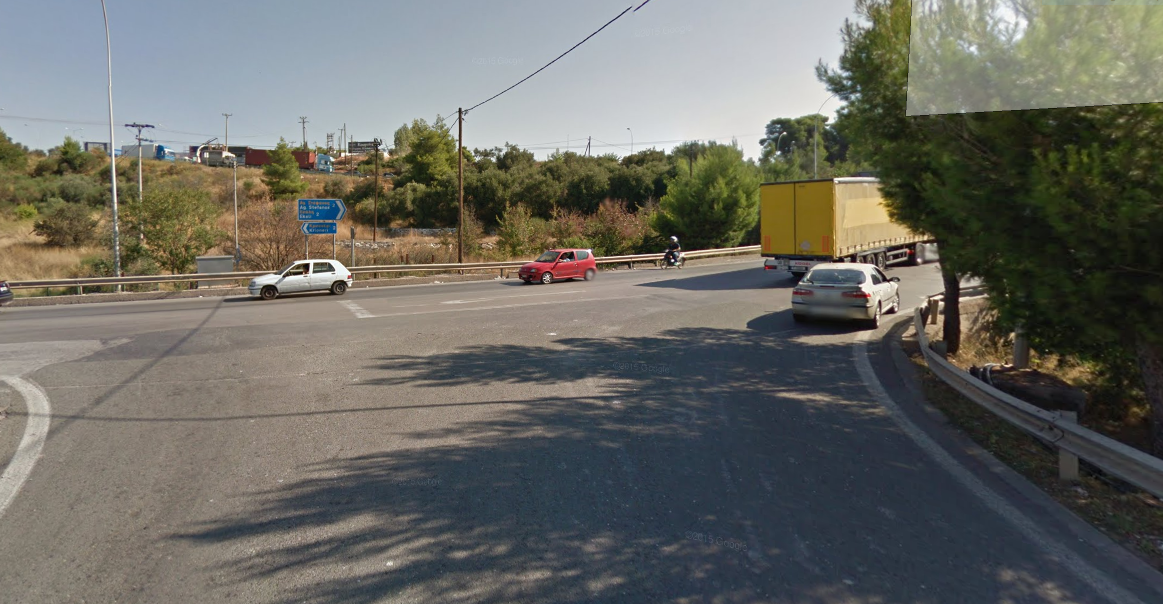
\includegraphics[width=\textwidth]{images/athina-lamia/astefanos/astefanos1.PNG}
			\caption{Στη διασταύρωση στρίβουμε δεξιά}
\end{figure}

Στη συνέχεια στο φανάρι στρίβουμε αριστερά, στην ανηφόρα και συνεχίζουμε ευθεία παράλληλα με την Εθνική οδό.

\begin{figure}[hbp!]
	\centering
		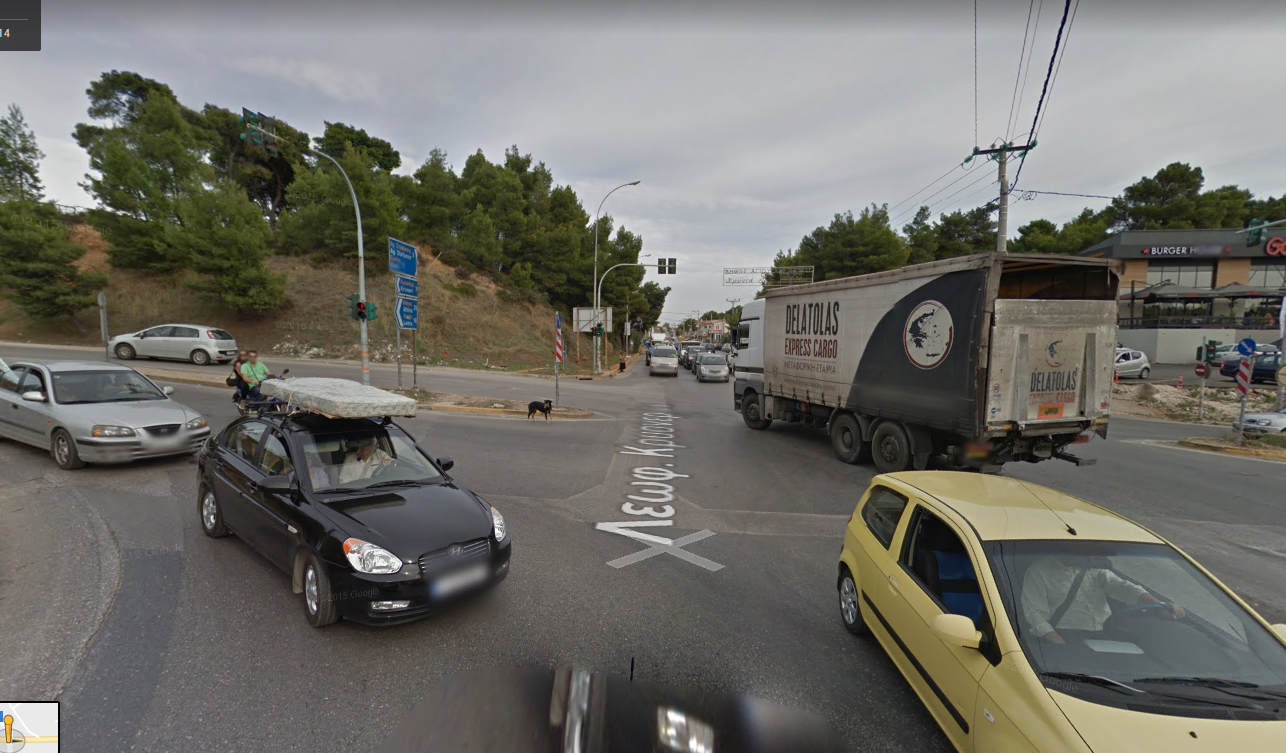
\includegraphics[width=\textwidth]{images/athina-lamia/astefanos/astefanos2.PNG}
			\caption{Μετά το φανάρι στρίβουμε αριστερά}
\end{figure}
\break
Συνεχίζουμε ευθεία μέχρι να περάσουμε αριστερά μας τα διόδια των Αφιδνών και στο τέλος του δρόμου φτάνουμε στη διασταύρωση όπου είναι τα ανθοπωλεία. Στρίβουμε αριστερά.

\begin{figure}[hbp!]
	\centering
		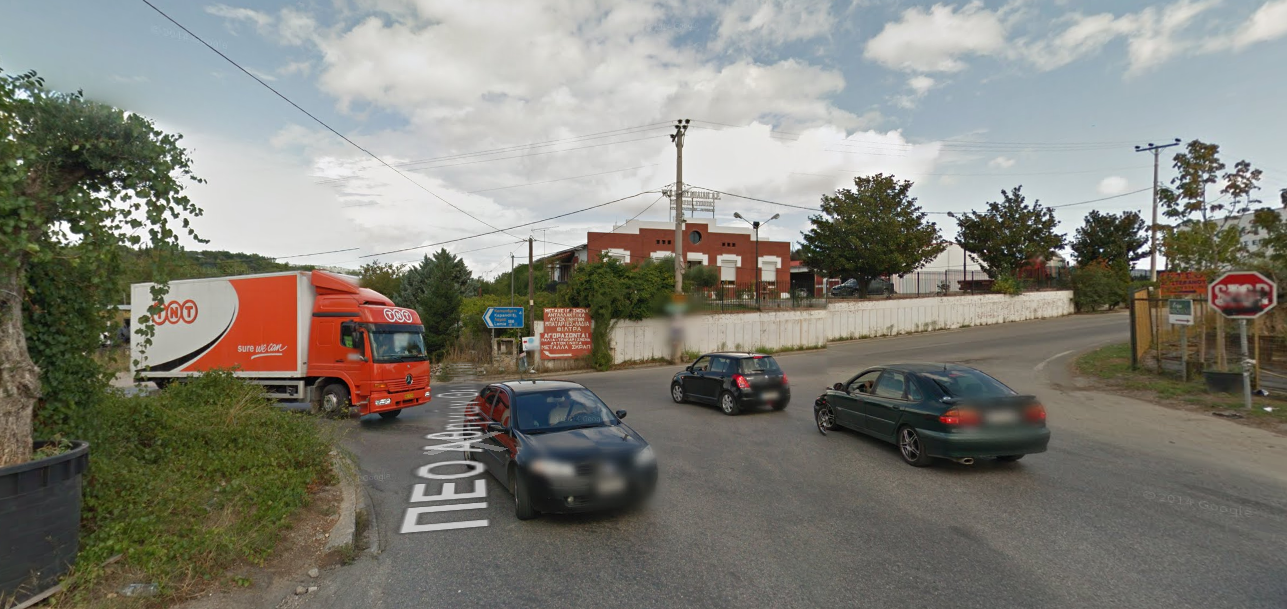
\includegraphics[width=\textwidth]{images/athina-lamia/astefanos/astefanos3.PNG}
			\caption{Στρίβουμε αριστερά}
\end{figure}
Συνεχίζουμε ευθεία μέχρι να φτάσουμε στη διασταύρωση της Μαλακάσας όπου και συνεχίζουμε ευθεία απέναντι (Ταμπέλα Αυλώνα 8) όπως και το φορτηγό βυτίο που φαίνεται στην εικόνα. \textbf{Προσοχή !!!}
Δεν πηγαίνουμε στην Αυλώνα αλλά προς την κατεύθυνση που πάει προς τα εκεί.  

\begin{figure}[hbp!]
	\centering
		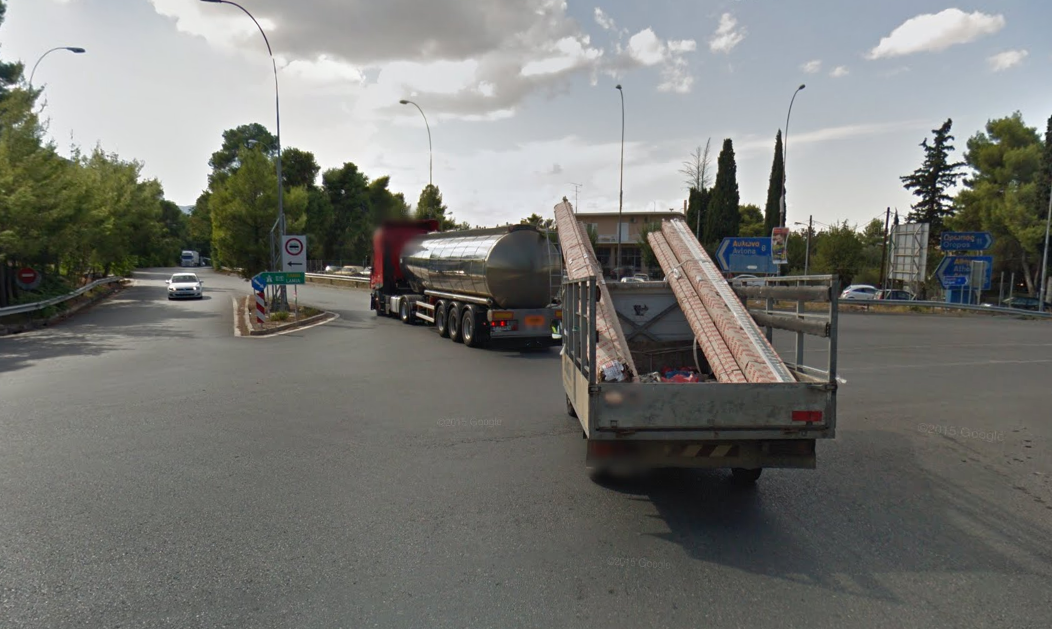
\includegraphics[width=\textwidth]{images/athina-lamia/astefanos/astefanos4.PNG}
			\caption{Κατευθυνόμαστε ευθεία απέναντι}
\end{figure}
\break
Δε στρίβουμε πουθενά και συνεχίζουμε ευθεία. Θα περάσουμε την είσοδο του στρατοπέδου στο δεξί μας χέρι και θα συνεχίσουμε ευθεία για αρκετό δρόμο μέχρι να φτάσουμε να δούμε ένα βενζινάδικο της Shell στο δεξί μας χέρι που έχει και αέριο. 
\begin{figure}[hbp!]
	\centering
		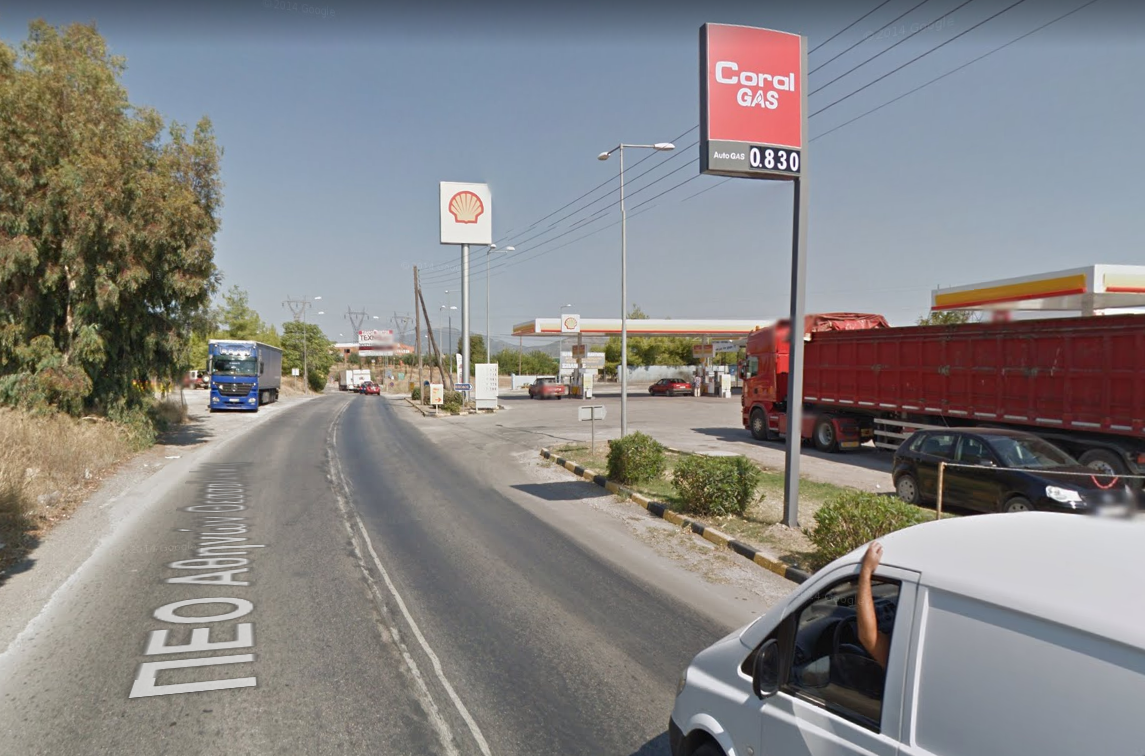
\includegraphics[width=\textwidth]{images/athina-lamia/astefanos/astefanos5.PNG}
			\caption{Το βενζινάδικο της Shell. Φτάνουμε στο κομμάτι που πρέπει να στρίψουμε}
\end{figure}

\break
Σε μερικές εκατοντάδες μέτρα θα φτάσουμε στη διασταύρωση που δεξιά πάει για Χαλκίδα(ένας καλός τρόπος για αποφυγή και για όσους ενδιαφέρονται να πάνε Χαλκίδα)και αριστερά για Σχηματάρι. Στρίβουμε αριστερά και αμέσως δεξιά όπως φαίνεται στις εικόνες.

\begin{figure}[hbp!]
	\centering
		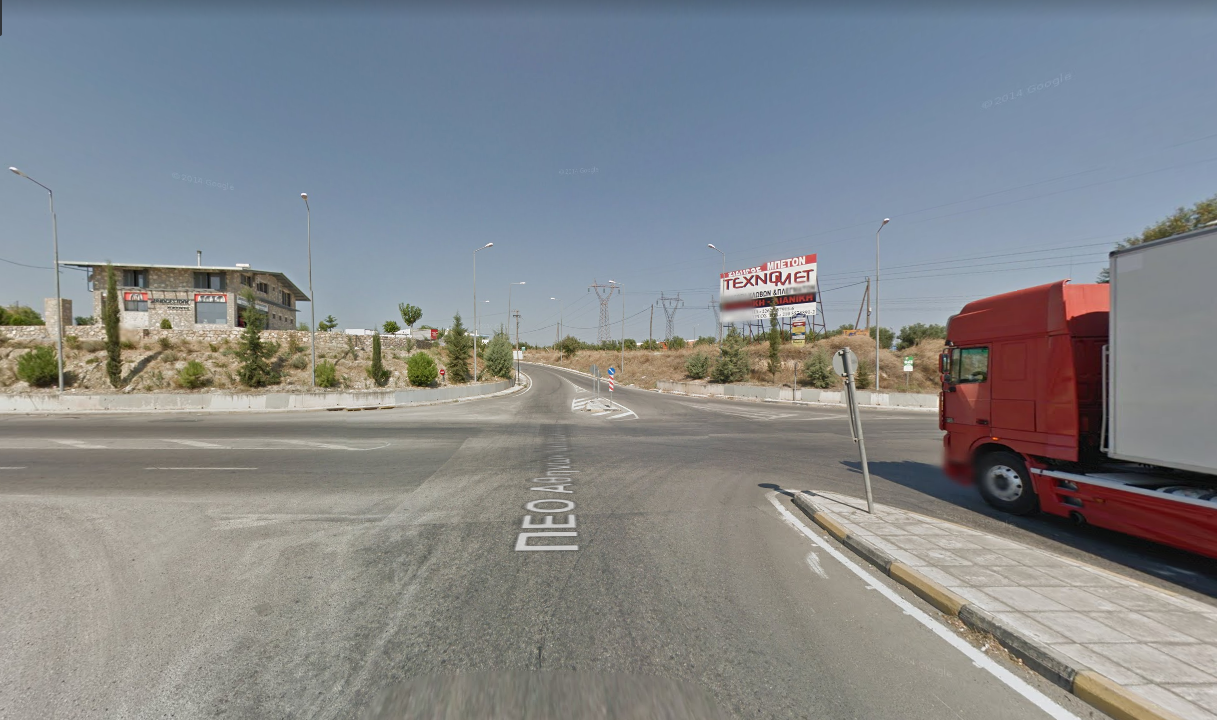
\includegraphics[width=\textwidth]{images/athina-lamia/astefanos/astefanos6.PNG}
			\caption{Στρίβουμε αριστερά και ...}
\end{figure}
\begin{figure}[hbp!]
	\centering
		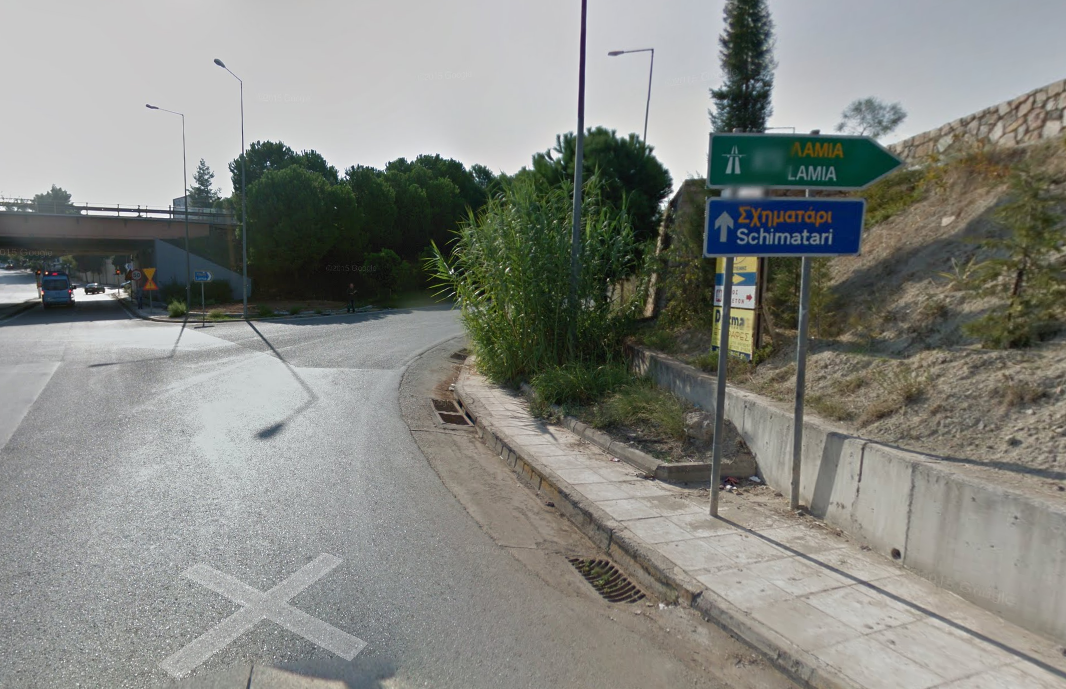
\includegraphics[width=\textwidth]{images/athina-lamia/astefanos/astefanos7.PNG}
			\caption{... αμέσως δεξιά στην ταμπέλα που λέει Λαμία}
\end{figure}

Βγαίνουμε στην Εθνική οδό.

\begin{center}
\section*{Αποφυγή διοδίων Θήβας}
\end{center}
\addcontentsline{toc}{subsection}{Αποφυγή διοδίων Θήβας}
Βρισκόμαστε στην Εθνική οδό και προχωράμε μέχρι να βρούμε την έξοδο για νοσοκομείο Θήβας.
\begin{figure}[hbp!]
	\centering
		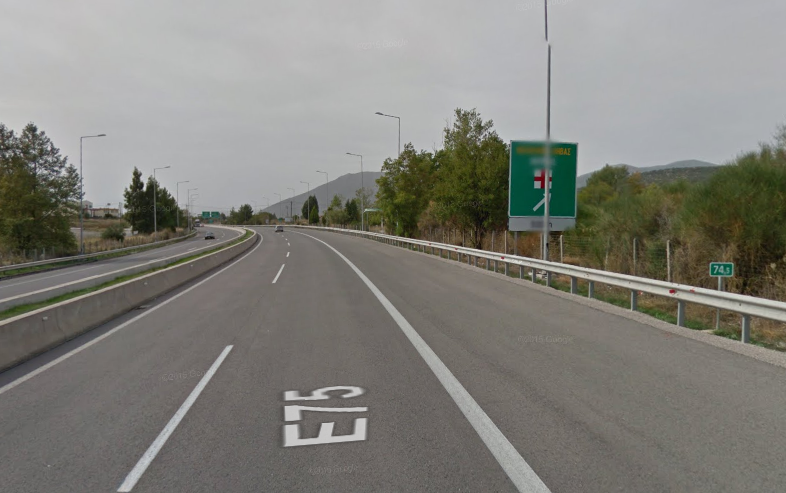
\includegraphics[width=\textwidth]{images/athina-lamia/thiva/thiva1.PNG}
			\caption{Μόλις δούμε την ταμπέλα στην επόμενη έξοδο πάμε δεξιά}
\end{figure}
Αφότου μπούμε συνεχίζουμε ευθεία απέναντι 
\begin{figure}[hbp!]
	\centering
		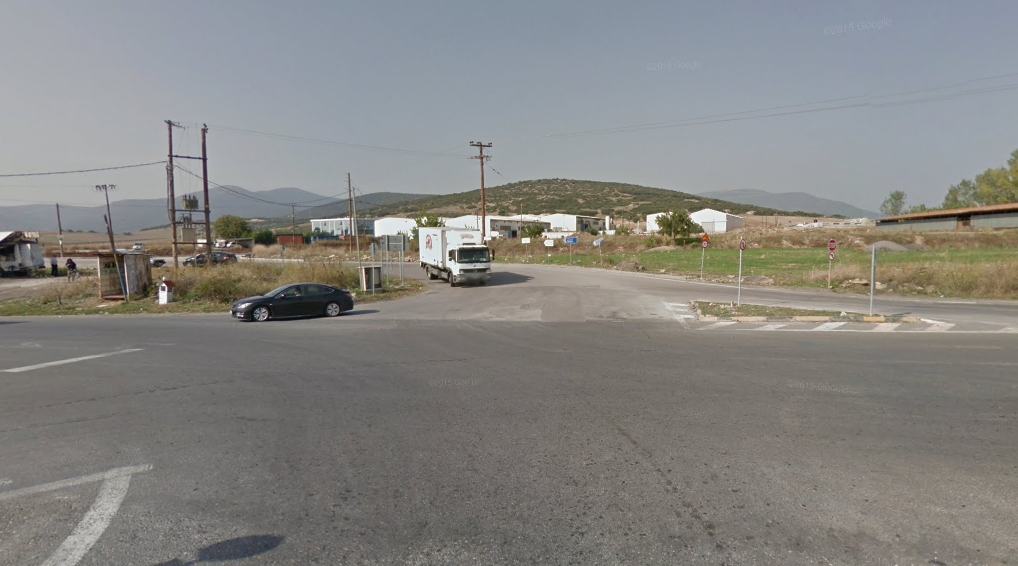
\includegraphics[width=\textwidth]{images/athina-lamia/thiva/thiva2.PNG}
			\caption{Πηγαίνουμε ευθεία απέναντι}
\end{figure}
\newpage
Καθ' όλη τη διάρκεια που θα είμαστε στον παράδρομο, θα έχουμε την Εθνική οδό στο αριστερό μας χέρι. Προορισμός μας είναι το καφέ 90, όπου από εκεί θα βγούμε ξανά στην Εθνική οδό. Στην πορεία θα συναντήσουμε 2 διασταυρώσεις όπου και στις 2 θα περάσουμε απέναντι. 
\begin{figure}[hbp!]
	\centering
		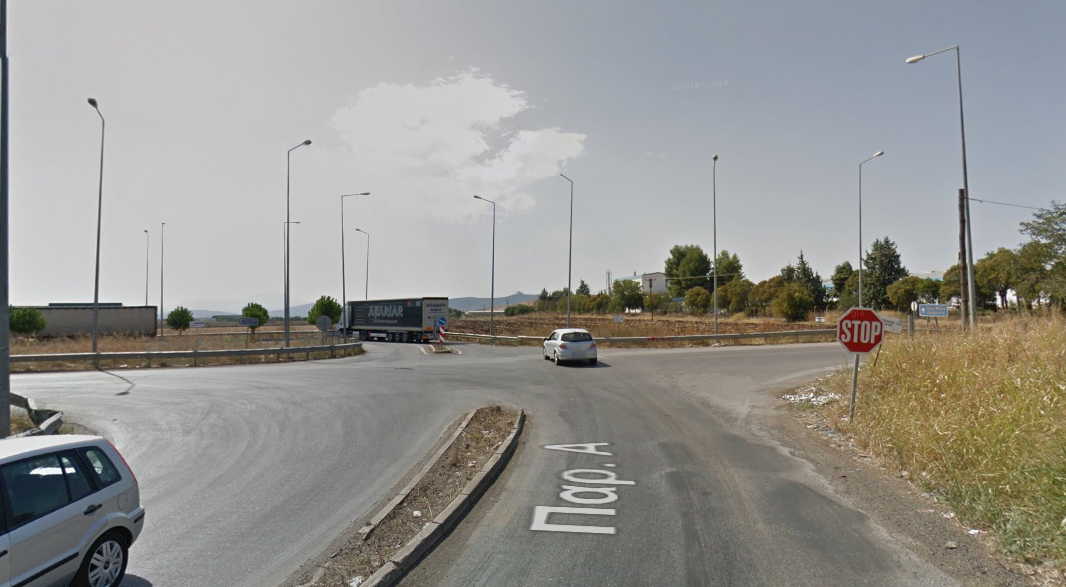
\includegraphics[width=\textwidth]{images/athina-lamia/thiva/thiva3.PNG}
			\caption{Πηγαίνουμε ευθεία απέναντι}
\end{figure}
\begin{figure}[hbp!]
	\centering
		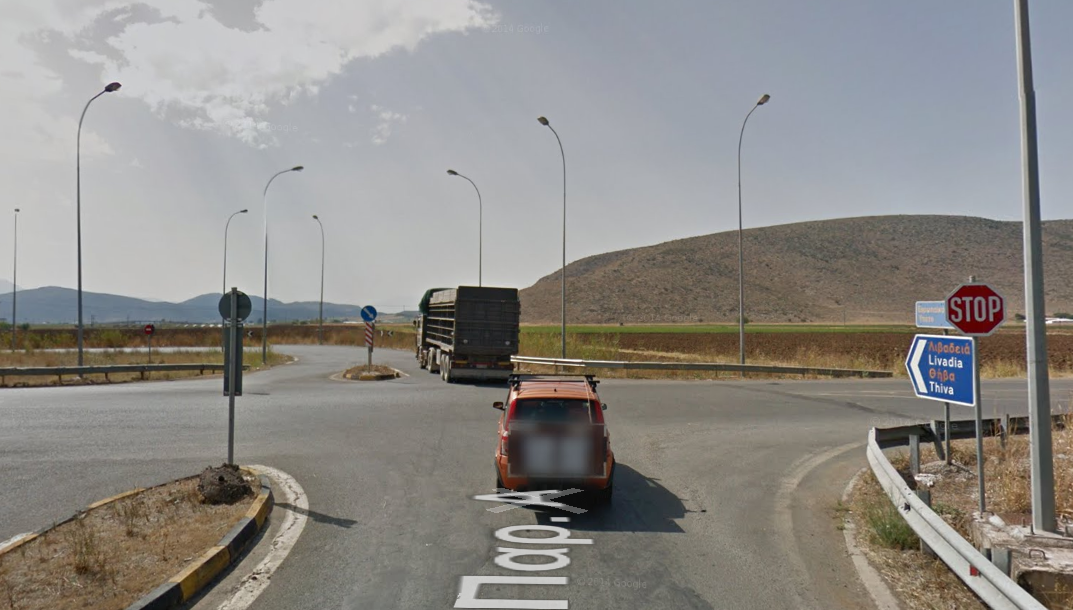
\includegraphics[width=\textwidth]{images/athina-lamia/thiva/thiva4.PNG}
			\caption{Συνεχίζουμε ευθεία απέναντι}
\end{figure}
Από εκεί και μετά συνεχίζουμε ευθεία μέχρι να μπούμε στο χώρο στάθμευσης του καφέ 90, από όπου βγαίνουμε στην Εθνική Οδό.
\newpage
\begin{center}
\section*{Αποφυγή διοδίων Τραγάνας}
\end{center}
\addcontentsline{toc}{subsection}{Αποφυγή διοδίων Τραγάνας}
Έχουμε βγει από το parking του καφέ 90 και βρισκόμαστε στην Εθνική οδό με κατεύθυνση προς Λαμία. Αφού περάσουμε το Κάστρο Βοιωτίας αναζητούμε την ταμπέλα που αναγράφει "Θεολόγος - Μαλαισίνα" και στην έξοδο στρίβουμε δεξιά.

\begin{figure}[hbp!]
	\centering
		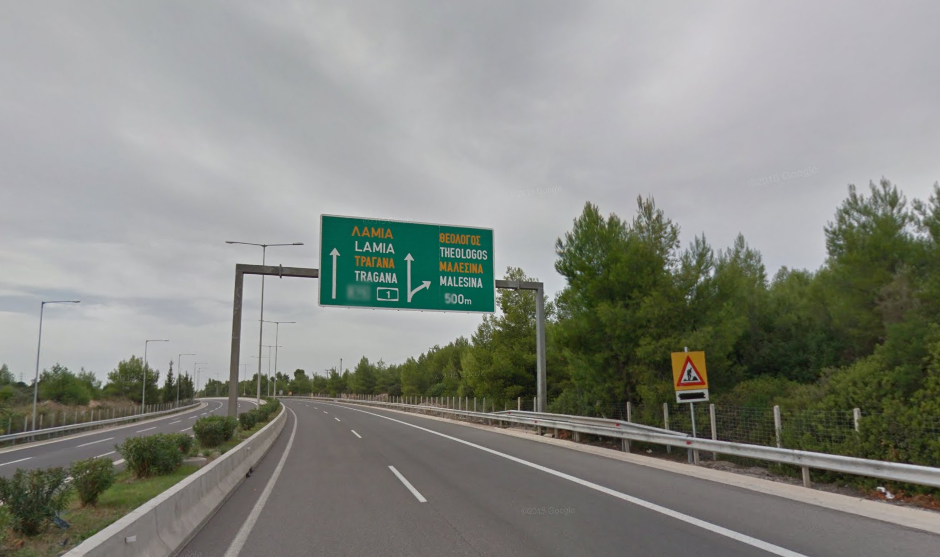
\includegraphics[width=\textwidth]{images/athina-lamia/tragana/tragana1.PNG}
			\caption{Στην έξοδο στρίβουμε δεξιά}
	
\end{figure}
\begin{figure}[hbp!]
	\centering
		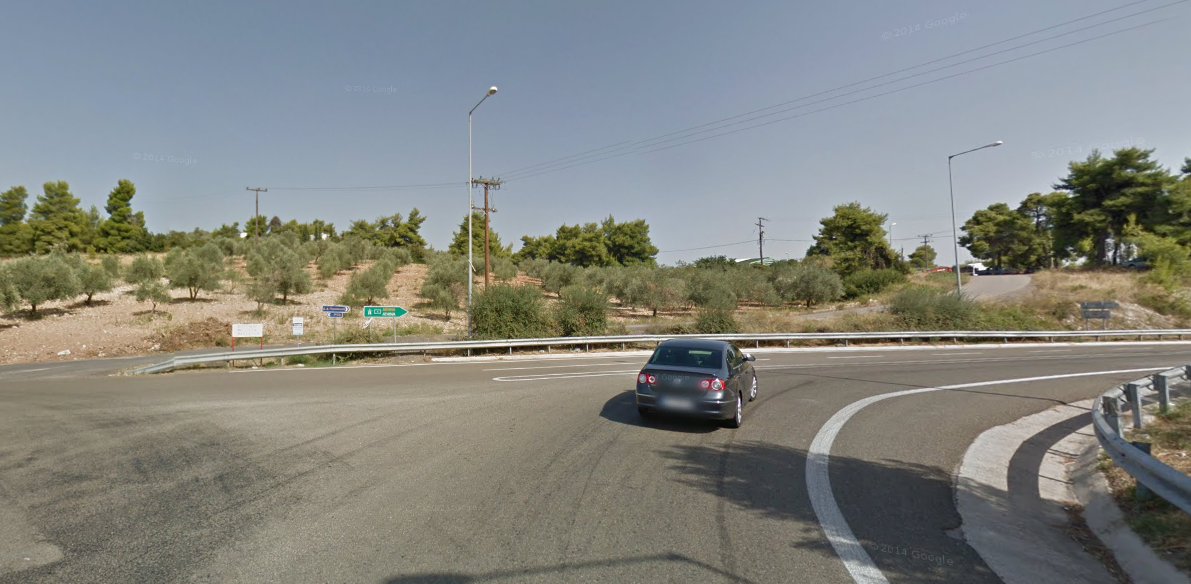
\includegraphics[width=\textwidth]{images/athina-lamia/tragana/tragana2.PNG}
			\caption{Στρίβουμε δεξιά (κατεύθυνση προς Προσκυνά)}
\end{figure}
\break			
Περνάμε κάτω από τη γέφυρα και κάνουμε αμέσως δεξιά. Η ταμπέλα γράφει Προσκυνάς-Θεολόγος και στα 50 μέτρα έχουμε στο αριστερό μας χέρι, ένα βενζινάδικο της Elin.

\begin{figure}[hbp!]
	\centering
		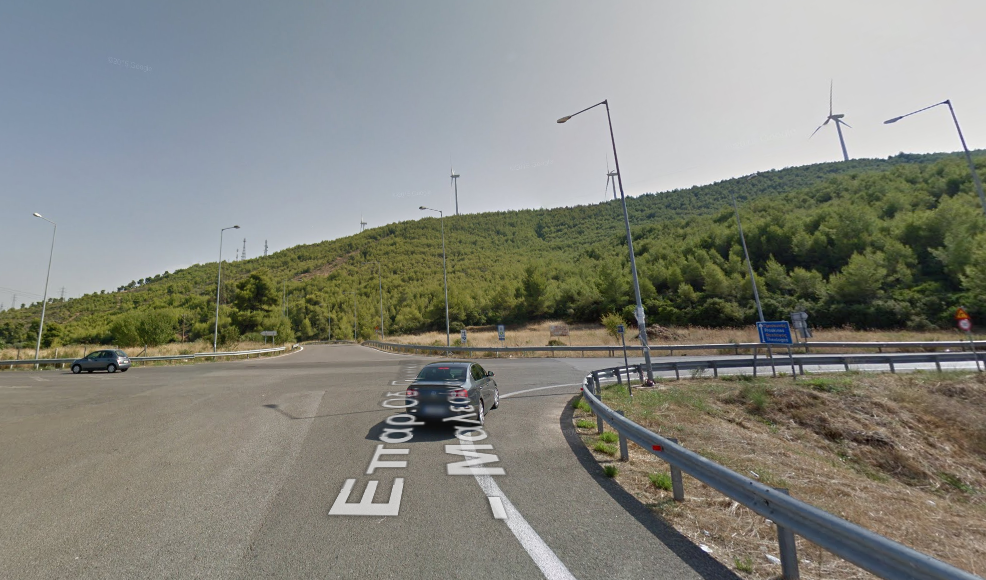
\includegraphics[width=\textwidth]{images/athina-lamia/tragana/tragana3.PNG}
			\caption{Στρίβουμε δεξιά (Ταμπέλες Προσκυνά-Θεολόγο)}
\end{figure}
Το επόμενο κομμάτι έχει μια μικρή δυσκολία στον εντοπισμό του, ειδικά αν δεν έχουμε ξανακάνει το δρόμο. Μόλις φτάσουμε στο σημείο της εικόνας θα κάνουμε αριστερά. Μέχρι να φτάσουμε εκεί δεν έχει κάποια ταμπέλα για αυτό καλό είναι να μην αναπτύξουμε μεγάλη ταχύτητα. Στρίβουμε αριστερά.
\begin{figure}[hbp!]
	\centering
		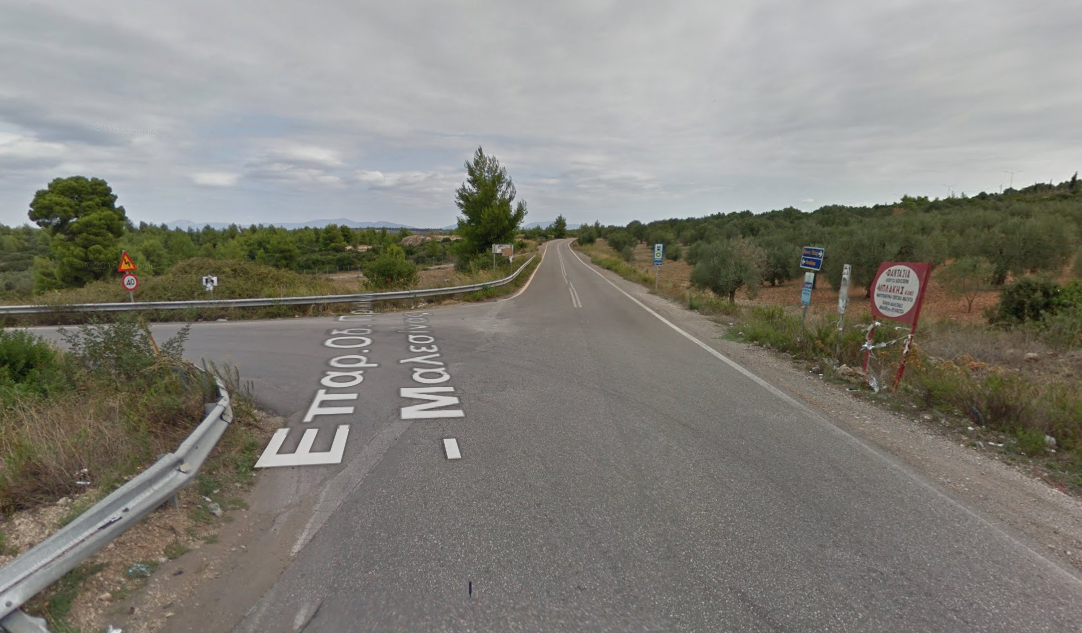
\includegraphics[width=\textwidth]{images/athina-lamia/tragana/tragana4.PNG}
			\caption{Στρίβουμε αριστερά}
\end{figure}
\newpage
Συνεχίζουμε ευθεία και φτάνουμε στο χωριό Προσκυνάς το οποίο και διασχίζουμε. Μόλις βγούμε από το χωριό κάνουμε διαγώνια αριστερά.
\begin{figure}[hbp!]
%	\centering
		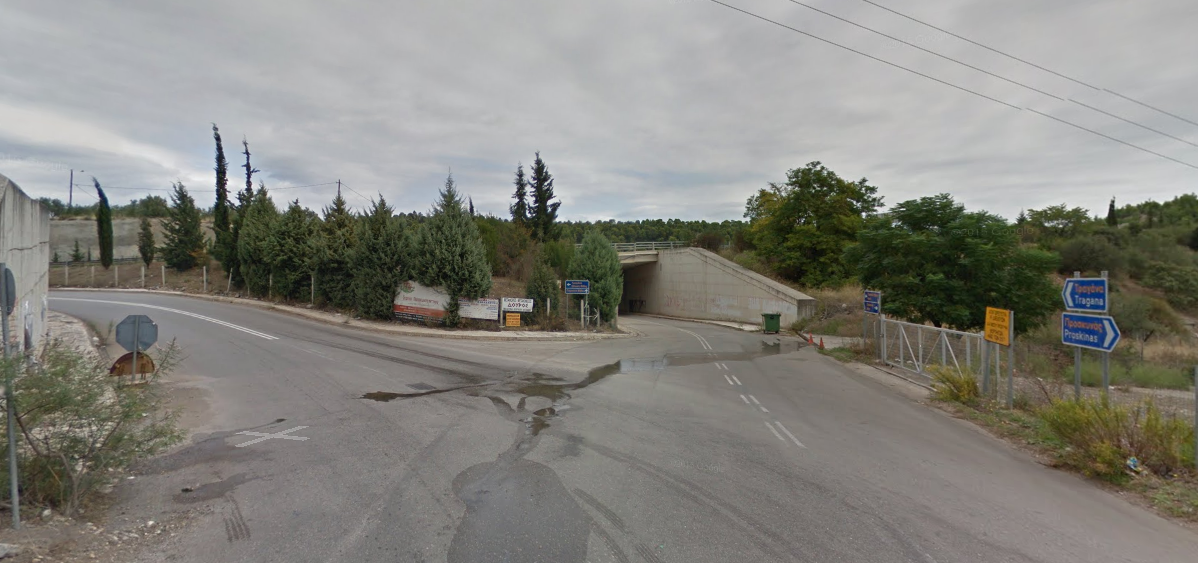
\includegraphics[width=\textwidth]{images/athina-lamia/tragana/tragana5.PNG}
			\caption{Στρίβουμε διαγώνια αριστερά}

%	\centering
		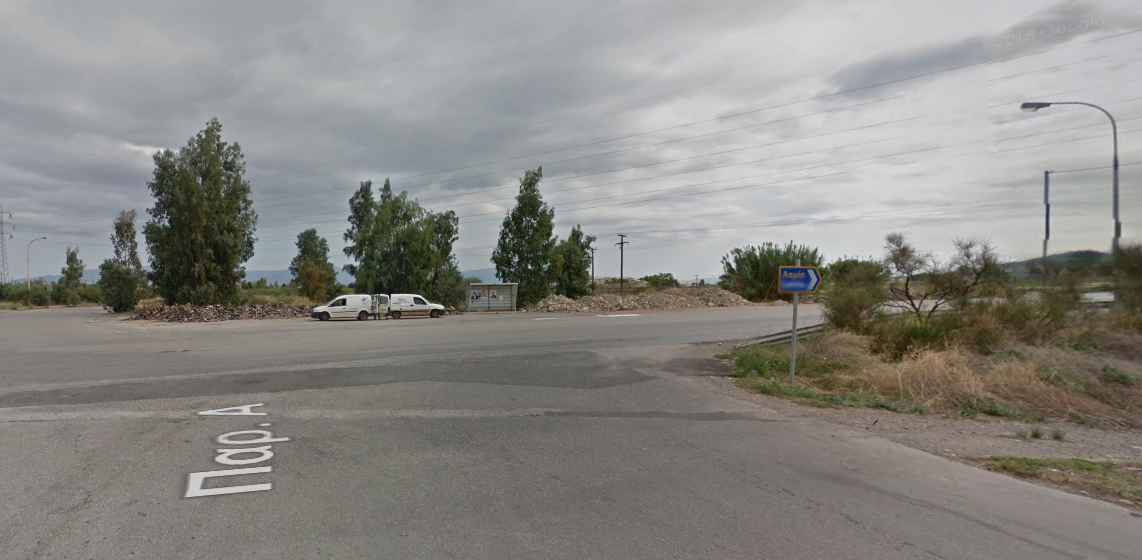
\includegraphics[width=\textwidth]{images/athina-lamia/tragana/tragana6.PNG}
			\caption{Στρίβουμε δεξιά (ταμπέλα προς Λαμία)}
\end{figure}			

Συνεχίζουμε ευθεία μέχρι να φτάσουμε στο τέλος του δρόμου, στη διασταύρωση της εικόνας. Στρίβουμε δεξιά (ταμπέλα προς Λαμία), περνάμε τη γέφυρα και αμέσως αριστερά. Ακολουθούμε το δρόμο και βγαίνουμε στην Εθνική οδό.

\begin{figure}[H]
		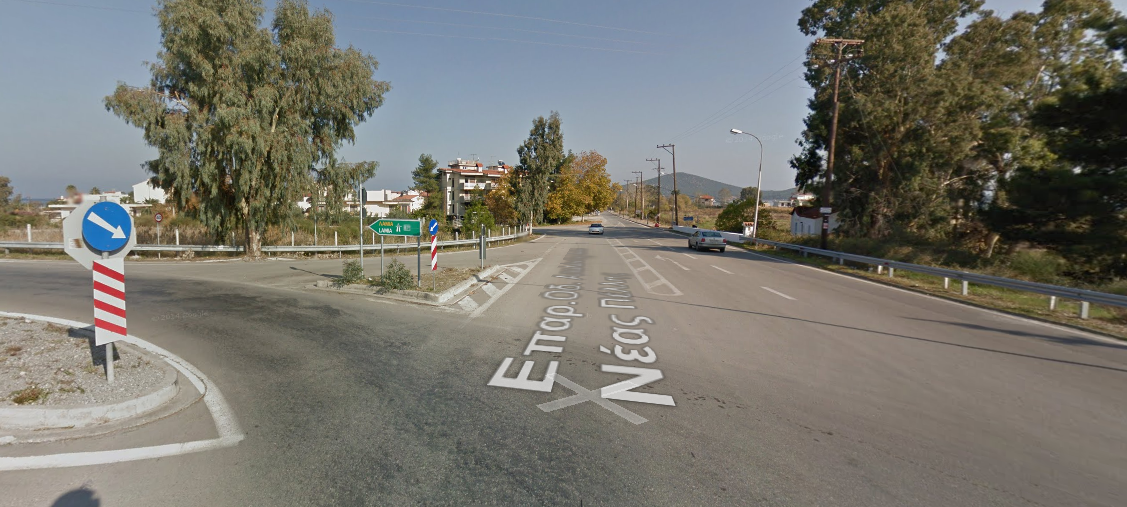
\includegraphics[width=\textwidth]{images/athina-lamia/tragana/tragana7.PNG}
			\caption{Στρίβουμε αριστερά (ταμπέλα προς Λαμία)}
\end{figure}
\newpage
\begin{center}
\section*{Αποφυγή διοδίων Λαμίας\footnote{Λαμβάνοντας υπόψη την αναλογία ταλαιπωρίας/αξίας κομίστρου, επιλέγουμε να πληρώσουμε το κόμιστρο του συγκεκριμένου σταθμού}}
\end{center}
\addcontentsline{toc}{subsection}{Αποφυγή διοδίων Λαμίας}
Βρισκόμαστε στην Εθνική οδό και αφού περάσουμε τις σύραγγες στο ύψος του Αγίου Κωνσταντίνου μόλις δούμε την ταμπέλα για Καμμένα Βούρλα, κάνουμε δεξιά και στη διασταύρωση αριστερά
		
\begin{figure}[H]
	\centering
		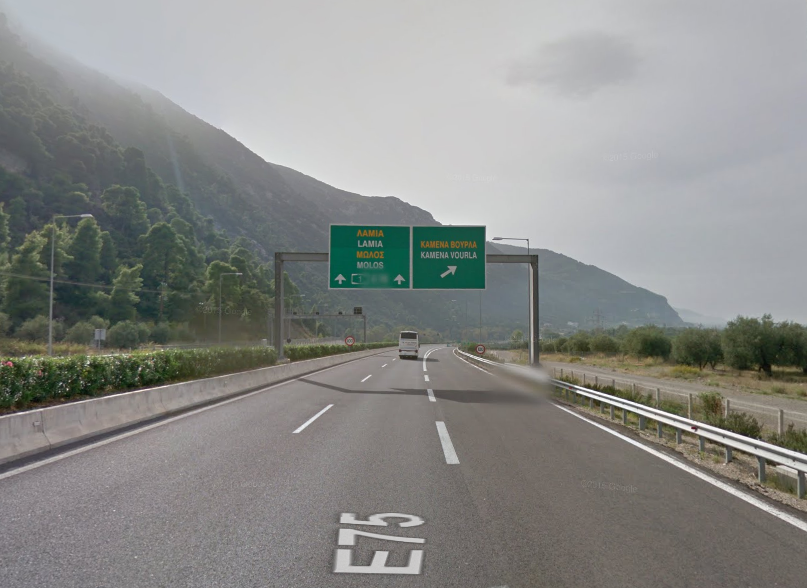
\includegraphics[width=\textwidth]{images/athina-lamia/lamia/lamia1.PNG}
			\caption{Μπαίνουμε στην έξοδο δεξιά}

	\centering
		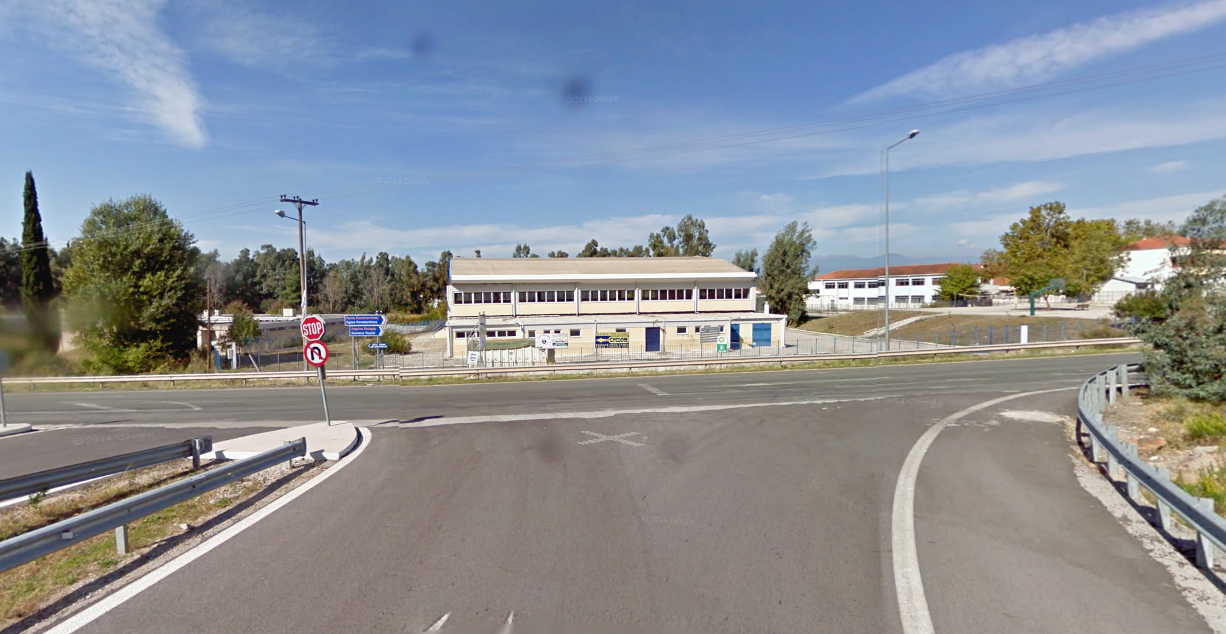
\includegraphics[width=\textwidth]{images/athina-lamia/lamia/lamia2.PNG}
			\caption{Στρίβουμε αριστερά στην ΠΕΟ (Παλιά Εθνική Οδό)}
\end{figure}
Συνεχίζουμε μέχρις ότου να φτάσουμε στη διασταύρωση που φαίνεται στην εικόνα. Στρίβουμε δεξιά κάτω από τη γέφυρα και μπαίνουμε στον κυκλικό κόμβο όπου κατευθυνόμαστε προς την κατεύθυνση που λένε οι ταμπέλες "Camping Ε.Ο.Τ."
\begin{figure}[H]
	\centering
		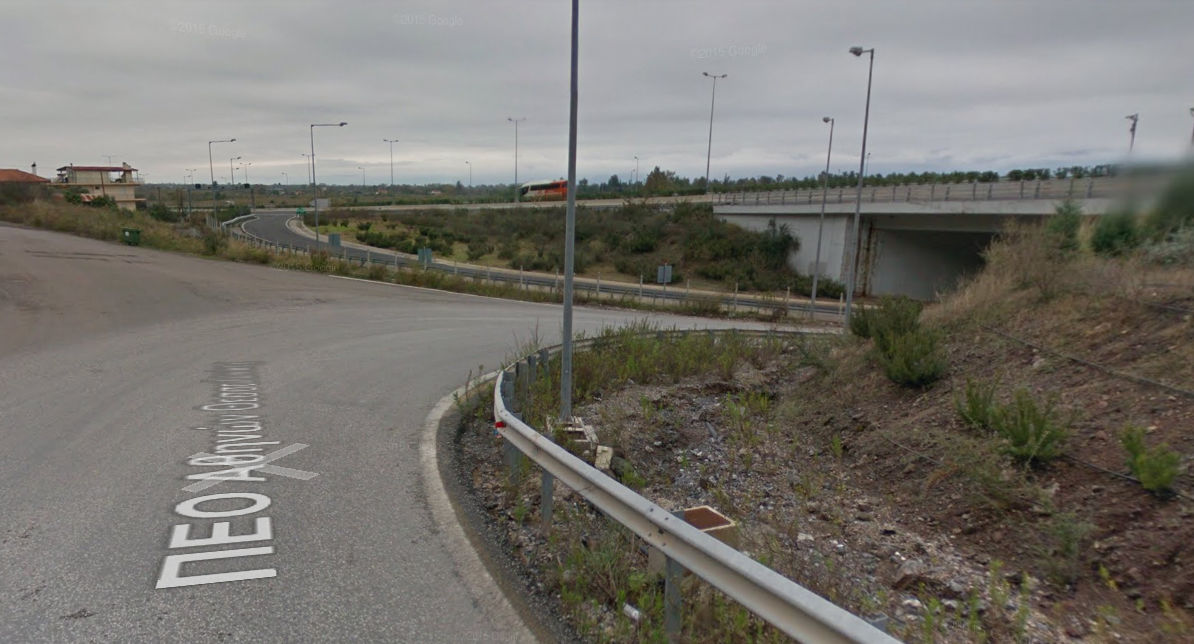
\includegraphics[width=\textwidth]{images/athina-lamia/lamia/lamia3.PNG}
			\caption{Κατευθυνόμαστε δεξιά κάτω από τη γέφυρα\newline}
	
	\centering
		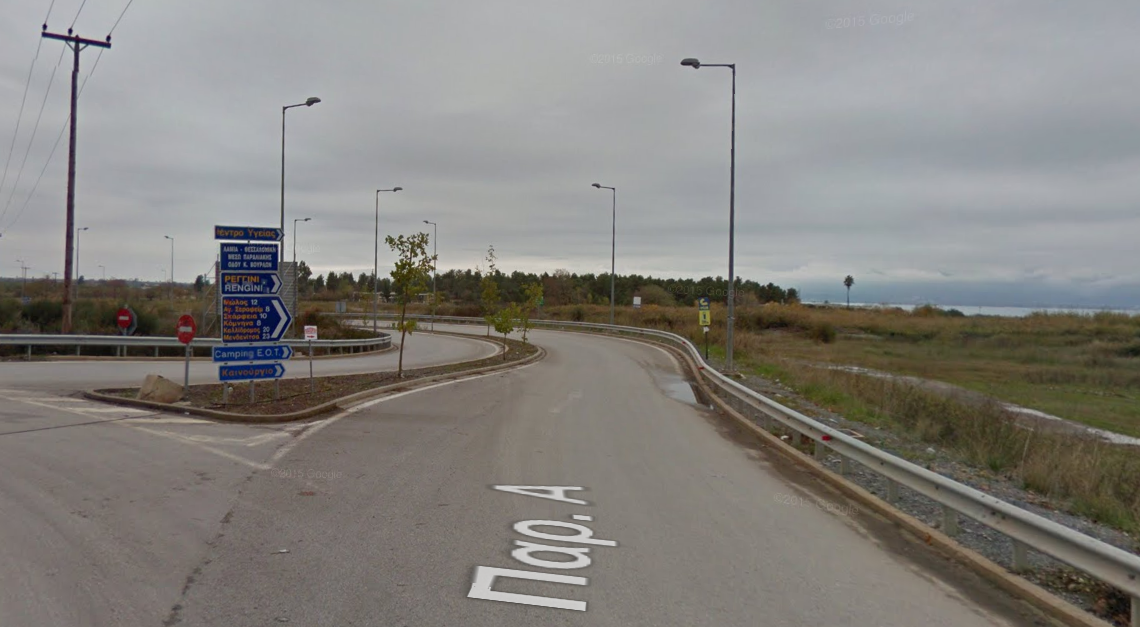
\includegraphics[width=\textwidth]{images/athina-lamia/lamia/lamia4.PNG}
			\caption{Πάμε προς την κατεύθυνση των ταμπελών}
\end{figure}
Προχωράμε ευθεία μέχρι να περάσουμε στο αριστερό μας χέρι τα διόδια της Λαμίας (Αγία Τριάδα). Περνάμε κάτω από την Εθνική οδό και ως εκ τούτου την έχουμε στο δεξί μας χέρι. Συνεχίζουμε ευθεία και περνάμε πάλι κάτω από την ΕΟ. Θα φτάσουμε σε ένα τριγωνικό κόμβο όπου θα συνεχίσουμε διαγώνια δεξιά. Συνεχίζουμε ευθεία μέχρι να βρεθούμε πίσω από τα Goody's της Λαμίας. Εκεί πηγαίνουμε διαγωνίως αριστερά όπως φαίνεται στην εικόνα και βγαίνουμε στην ΕΟ.
\begin{figure}[H]
	\centering
		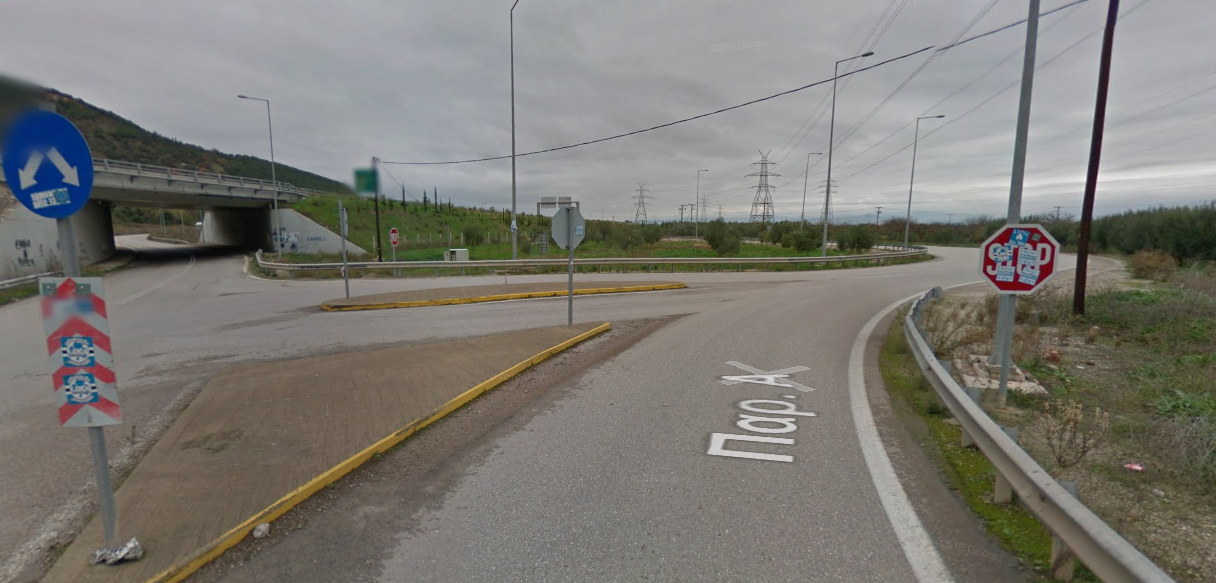
\includegraphics[width=\textwidth]{images/athina-lamia/lamia/lamia5.PNG}
			\caption{Κατευθυνόμαστε δεξιά στον κόμβο}
	
	\centering
		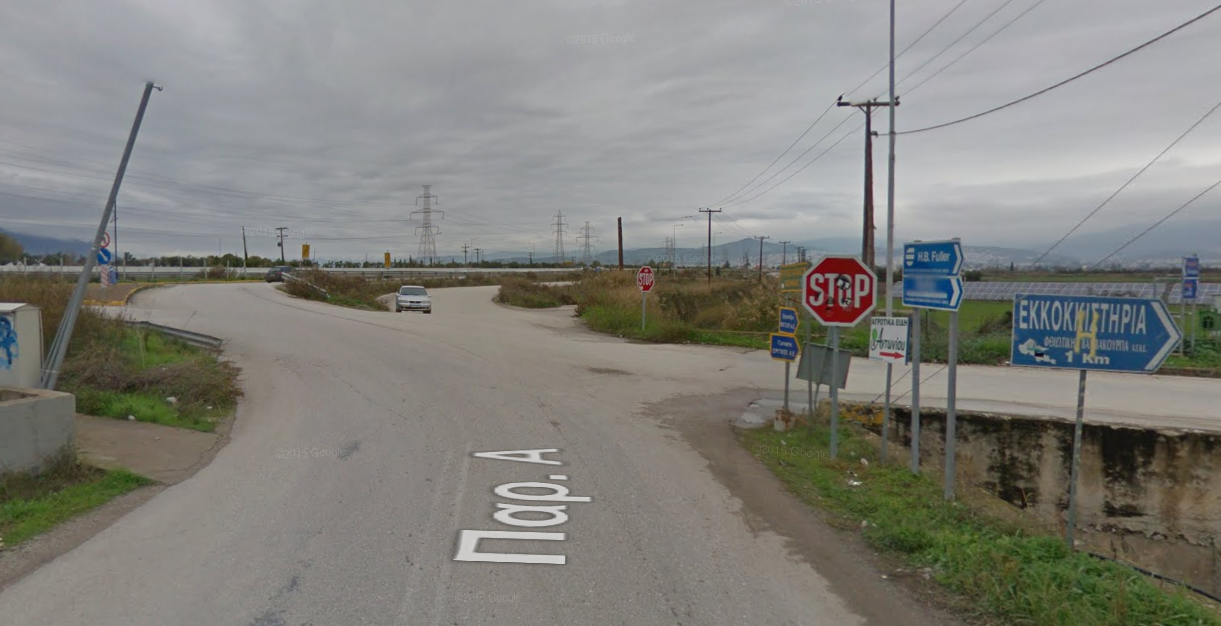
\includegraphics[width=\textwidth]{images/athina-lamia/lamia/lamia6.PNG}
			\caption{Προχωράμε διαγώνια αριστερά}
\end{figure}

Είμαστε στην ΕΟ και σε λίγο φτάνουμε Λαμία. Αν συνεχίσουμε ευθεία για Βόλο,Λάρισα,Θεσσαλονίκη θα συναντήσουμε διόδια. Μπορούμε όμως στρίβοντας δεξιά να πάμε χωρίς επιβάρυνση προς Καρδίτσα,Τρίκαλα αλλά και Λάρισα καθώς και Βόλο (μέσω Φαρσάλων).
\vspace{12pt}
\paragraph{Μέχρι τη Λαμία εξοικονομήσαμε}
\begin{itemize}
\item Αυτοκίνητο = 12.60€
\item Μηχανή = 8.75€
\item Φορτηγό ή μικρό ρυμουλκούμενο = 31.55€
\item Νταλίκα = 44.2€
\end{itemize}
\newpage
